\subsection{Unification-Based Points-to Analysis}
\label{sec:points-to}

Many program analysis tools~\citep{bddbddb, cclyzer, doop}
 are implemented in Datalog.
The declarative nature of Datalog makes the development easier,
 and the mature relational query optimization and execution techniques
 provide competitive performance and
 sometimes lead to order-of-magnitude speedup~\citep{doop}.

Points-to analysis
 computes an over-approximation of 
 the set of possible allocations a pointer can point to at run time.
% Most points-to analyses implemented in Datalog 
%  are subset based (i.e., Andersen style~\cite{andersen1994program}).
% In a subset based analysis, 
%  $\mathsf{points\_to}(p, a)$
%  is a relation that says pointer $p$ may point to allocation $a$.
% A pointer may point to many distinct allocations.
% These analyses are precise but scale poorly.
% Transitivity of $\mathsf{points\_to}$ gives rise to quadratic complexity:
%  if $\mathsf{points\_to}(p_1, a_1)$ and $\mathsf{points\_to}(p_2, a_2)$,
%  then the analysis must also record that that $\mathsf{points\_to}(p_1, a_2)$.
Most points-to analyses implemented in Datalog 
 are subset based (i.e., Andersen style).
These analyses are precise, 
 but they scale poorly due to its quadratic complexity.
On the other hand, 
 unification-based points-to analysis (i.e., Steensgaard style~\cite{DBLP:conf/popl/Steensgaard96})
 is nearly linear in complexity
 and therefore scales much better,
 at the cost of potential imprecision.
% In a unification-based analysis,
%  $\mathsf{points\_to}$
%  is essentially a \emph{function} from pointer $p$ to allocation $a$.
In a unification-based analysis,
 if it is ever learned that $p$ 
 may point to two allocations $a_1$ and $a_2$,
 the allocations are \emph{unified} and considered equivalent.
The points-to relation in a Steensgaard analysis
 is essentially a function from pointers to the equivalence class of allocations
 they point to.
This is less precise than subset-based analysis,
 but it is more scalable, 
 because it avoids tracking every individual allocation a pointer points to.

However, despite its success in hosting other program analysis algorithms, 
 classical Datalog fails to express Steensgaard analysis efficiently
 due to the lack of support for fast equivalence.
A plain representation of the equivalence relation in Datalog 
 is quadratic in space, 
 which defeats the purpose of unifying points-to allocations of a pointer.
Recently, \souffle added support for union-find--backed relations
 to benefit from the space- and time-efficient representation 
 in the union-find data structure~\citep{eqrel}.
Relations marked with the \eqrel keyword in \souffle will be stored using union-find,
 so the equivalence closure property of the relation will be automatically maintained,
 without explicit rules like transitivity, which is quadratic.
However, \eqrel relations in \souffle 
 only \emph{maintain} equivalence relations efficiently,
 but fail to interact with the rest of the rules efficiently.
Therefore,
 practical Steensgaard analyses do not use the equivalence relation directly.
Consider this rule\footnote{In contrast to our paper, 
 \citet{eqrel} views \lstinline[language=Souffle]{vpt} itself as an \eqrel relation, 
 and the body of the rule joins over only 
 \lstinline[language=Souffle]{store}, \lstinline[language=Souffle]{vpt}, \lstinline[language=Souffle]{load}.
 Our presentation here is adjusted to be consistent with \cclyzerpp.} adapted from the Steensgaard analysis benchmark 
 in the \eqrel paper~\citep{eqrel}:
\begin{lstlisting}[language=Souffle]
// *x = y; p = *q; x and q points to the same set of allocs
eql(yAlloc, pAlloc) :- store(x, y), vpt(x, xAlloc), vpt(y, yAlloc),
                       load(p, q), vpt(p, pAlloc), vpt(q, qAlloc), 
                       eql(xAlloc, qAlloc),
\end{lstlisting}
where \verb|vpt| is the points-to relation from pointers to allocations,
 and \verb|eql| is the equivalence relation declared with \eqrel.
To see the performance of this rule,
 let us consider the subquery \lstinline[language=Souffle]{vpt(x, xAlloc), vpt(q, qAlloc), eql(xAlloc, qAlloc)}.
To evaluate this subquery,
 \souffle has to join over the \lstinline[language=Souffle]{eql} relation, 
 even when it is known that \lstinline[language=Souffle]{xAlloc} and \lstinline[language=Souffle]{qAlloc} are equivalent.
We call this additional join over the equivalence relation ``join modulo equivalence''.
This occurs frequently when using equivalence relations in practice 
 and often leads to unacceptable performance.
\Egglog eliminates this join modulo equivalence 
 by actively canonicalizing each element to its canonical representation.
Because two elements are equivalent if and only if they have the same canonical representation,
 it suffices for \egglog to perform only an equality join 
 over \lstinline[language=Souffle]{vpt(x, xAlloc)} and \lstinline[language=Souffle]{vpt(q, qAlloc)} with \lstinline[language=Souffle]{qAlloc = xAlloc},
 without joining with an auxillary quadratic relation.

\cclyzerpp~\citep{cclyzerpp,cclyzer} implements Steensgaard analyses in Datalog with extensions,
 \souffle in particular.
Joins like the above are too expensive for \cclyzerpp, 
 so \cclyzerpp avoids such joins modulo equivalence as much as possible.
In fact, 
 profiling shows that 
 the only rule that involves join modulo equivalence in \cclyzerpp
 is an order of magnitude slower 
 than any other rule \cclyzerpp uses to compute the points-to analysis.
%  \yz{with the caveat that the most time-consuming rules, which are the three triangle queries,
%  are used to compute alias analysis, not points-to analysis}

In Steensgaard analyses, 
 all allocations pointed to by the same pointer should be unified,
 so only one allocation per pointer will need to be tracked,
 which ensures an almost linear performance.
However,
 this key performance benefit 
 is lost in a direct encoding of Steensgaard analyses
 in Datalog.
For each pair of pointer \lstinline[language=Souffle]{p} 
 and the allocation it points to,
 a direct encoding will create a tuple \lstinline[language=Souffle]{vpt(p, alloc)},
 so \lstinline[language=Souffle]{vpt} may contain many allocations pointed to 
 by the same pointer, despite them all being equivalent.
The many allocations pointed to by the same pointer
 will be further propagated to other pointers,
 causing a blow up in the points-to relation.
To make sure only 
 one representative per equivalence class will be 
 propagated, \cclyzerpp uses a complex encoding
 with choice domain~\citep{choice-datalog, choice-souffle}
 and customize its own version of equivalence relation using 
 subsumptive rules~\citep{datalog-subsumption}.

Qualitatively, 
 we argue such an encoding is complex and error-prone,
 and we identify two independent bugs 
 related to the \cclyzerpp encoding.
%  of customized equivalence relation 
%  and the encoding of congruence 
%  when reimpelemnting their encoding for the benchmark on pointer analyses.
Each bug could lead to unsound points-to analysis result.
To fix the bugs, 
 we have to bring back the \eqrel relations of \souffle.
In other words, our patched version involves 
 the interaction among choice domain, subsumptive rules, 
 and \eqrel relations, three of the newest features of \souffle.
In our experience,
 the interplay of these features can produce unexpected results
 and is extremely tricky to debug.

Compared to the sophisticated and unintuitive encoding 
 one has to develop to express efficient Steensgaard analyses
 in Datalog,
 writing Steensgaard analyses in \egglog is straightforward.
The user only needs to specify that the \lstinline[language=Souffle]{vpt} relation is 
 a function where functional dependency repair is done via 
 unifying the violating ids,
 and \egglog takes care of 
 all the unification and canonicalization.
Our insight here with \egglog is that,
 if two terms are known to be equivalent,
 they should considered indistinguishable by
 the database. 
\Egglog's canonicalization
 means we do not have to join modulo equivalence;
 a regular join suffices.

\paragraph{Benchmarking Points-To Analysis}

\begin{figure}
  \centering
  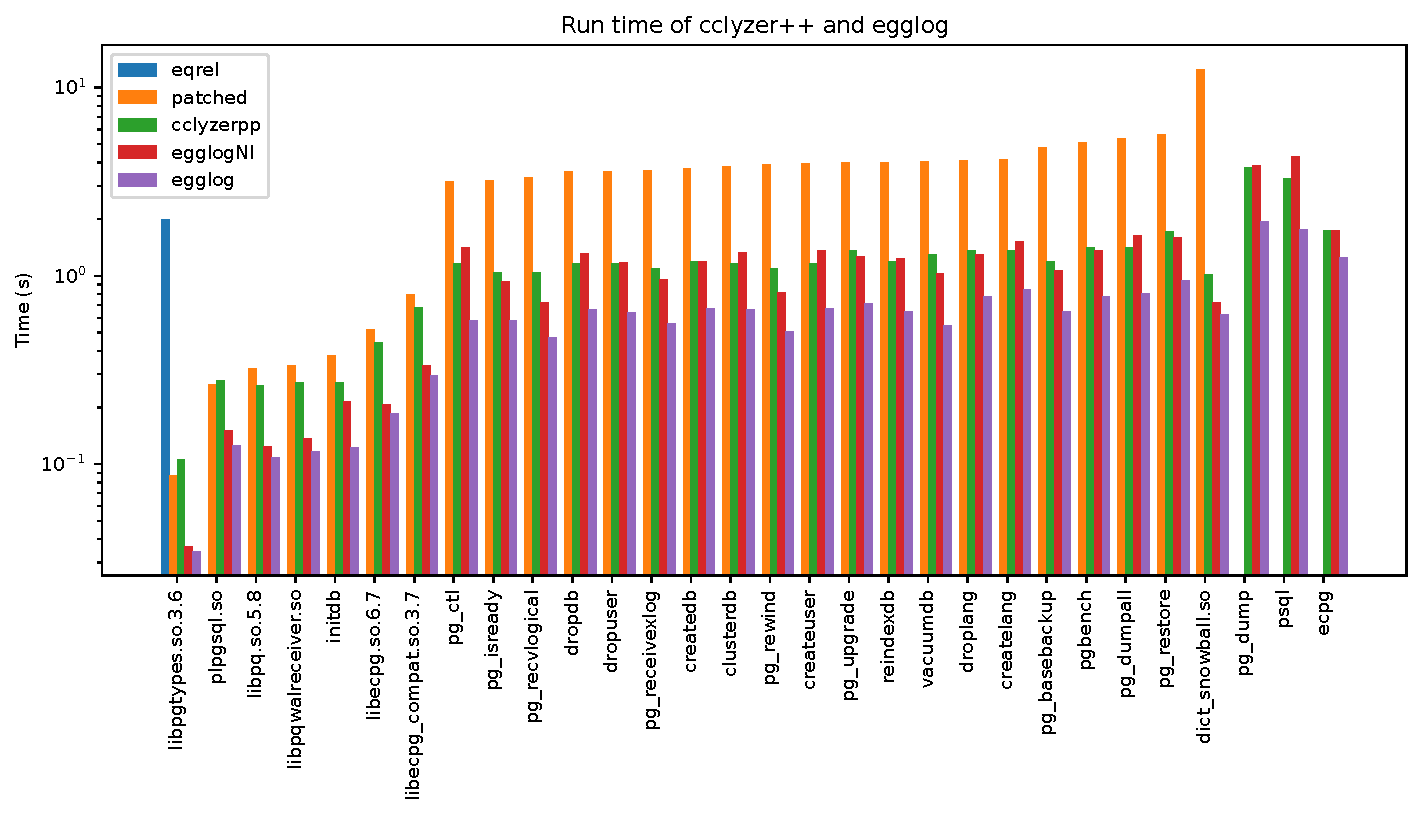
\includegraphics[width=\linewidth]{figs/pointer-analysis.pdf}
  \caption{
    Performance comparison between \egglog and various encoding 
    of Steensgaard analyses in Souffl\'e.
    Benchmarks that time out are not shown.
    In particular, \eqrel times out on all 
    but one benchmarks and \cclyzerpp times out
    on the three benchmarks on the right.}
  \label{fig:points-to}
\end{figure}

We benchmark the performance of \egglog on points-to analyses 
 against three baselines: 
\begin{itemize}
    \item \eqrel
     uses an explicit \eqrel relation to represent
     the equivalences among allocations.
     In \eqrel, because there is no canonical representation of pointers,
      a pointer may point to multiple (equivalent) allocations in \lstinline{vpt}.
    \item \cclyzerpp uses the original encoding \cclyzerpp
     developed for Steensgaard analyses.
    It uses a custom equivalence relation 
     that keeps record of the canonical representation of an allocation
     and avoids duplicated allocations 
     with \souffle's choice domain feature.
    However, \cclyzerpp has to perform joins modulo equivalence 
     for analyzing the \lstinline{load} instruction,
     and the custom equivalence relation is semantically unsound.
   \item \texttt{patched} is a patched encoding we developed based on \cclyzerpp's encoding.
   We made the custom equivalence relation sound by bringing back the \eqrel relation in \souffle,
    while keeping the canonical representations of allocations.
   We also added an additional rule to address a congruence-related bug in \cclyzerpp.
\end{itemize}
Moreover, we compare against 
 \texttt{egglogNI}, the non-incremental variant of \egglog with semi-na\"ive disabled.

We reimplemented a subset of \cclyzerpp in \egglog and three baselines. 
The points-to analyses we implement is context-, flow-, path-insensitive and field-sensitive.
% We ran \egglog and the three baselines on programs from two projects, coreutils-8.24 and postgresql-9.5.2.
We ran points-to analyses written 
 in two variants of \egglog and the three baselines 
 on programs from postgresql-9.5.2 with a timeout of 20 seconds.
All the systems except for \cclyzerpp 
 report the same size for computed points-to relations.
% Moreover, all the systems except for \cclyzerpp 
%  reports the same size for computed points-to relations.
\autoref{fig:points-to} shows the result.
\eqrel times out on all but one of the benchmarks, 
 and the patch to \cclyzerpp, despite making it sound,
 does make the encoding slower with the explicit equivalence relation
 and times out on three of the benchmarks.
\texttt{egglog} is faster than all Souffl\'e based baselines.
The comparison between \texttt{egglog} and \texttt{egglogNI}
 additionally shows that semi-na\"ive evaluation brings a substantial amount of 
 speedup to the computation of points-to analyses 
 by avoiding duplicated works.
Not counting the timed-out benchmarks, 
 \texttt{egglog} achieves a 4.96$\times$ speedup over \texttt{patched} on average,
 which is the fastest sound encoding in \souffle available.
Moreover, it achieves a 1.94$\times$ speedup over \cclyzerpp, 
 and 1.59$\times$ over \texttt{egglogNI}.
